\section{项目的主要内容和技术路线}

\subsection{主要研究内容}
根据心理学研究中常用的情绪分类模型和情绪生理机制,本研究主要聚焦的情绪种类为负性情绪-恐惧、正性情绪-愉悦和中性情绪-平静,相应采集的外周生理信号包括心电、脉搏波和呼吸信号,
旨在通过以上三种外周生理信号实现对部分基本情绪的识别。项目的主要内容包括以下四个部分:
(1)情绪刺激材料评价实验的方案设计与数据收集、处理;(2)情绪生理唤醒实验的方案设计与信号采集;(3)信号处理与特征提取;(4)模型构建与验证。

\subsection{技术路线}
\subsubsection{情绪刺激材料评价实验}
\begin{enumerate}[\hspace{2em}1.]
    \item 方案设计
\end{enumerate}

对于情绪诱发范式,论文将选用研究中较为常用的电影片段诱发方式,除平静视频外每种情绪至少选择5个视频片段作为备选,视频范围主要参考DECAF数据库\cite{DECAF2015}。考虑到视频片段的情绪诱发效果受个体差异影响较大,同时还存在国内外的文化差异影响,
在情绪生理唤醒实验前设置情绪刺激材料的评价实验,招募一定数量的被试(需满足心理学30人大样本的要求)观看顺序随机的视频组(同种情绪类型的视频不连续出现,每个视频间隔一定的休息时间),并在每个视频结束时填写:
1)自我评估量表,评价视频的唤醒度、效价和支配度(9点视觉量表),喜爱程度和熟悉程度(9点文字量表,1=“一点也不”,9=“极端”)以及是否有回避行为(2点文字量表,1=“是”,2=“否”),以分析每个视频在效价-唤醒模型中的分布情况,
并进行相关统计学检验;2)情绪评价量表,评价视频对每种基本情绪的诱发效果(9点文字量表,1=“一点也不”,9=“极端”),以分析每个视频对目标情绪的命中率和平均诱发强度是否达到标准。实验最后,被试还应填写一份测量抑郁、焦虑程度的问卷(包括抑郁PHQ-9、焦虑GAD-7、心理疾病史和住院史),以辅助后续的数据分析。

\begin{enumerate}[\hspace{2em}2.]
    \item 实验程序设计
\end{enumerate}

根据情绪刺激材料评价实验的方案设计,我将参与完成实验中需要使用的Python程序,界面主要包括各视频播放界面、量表界面、休息界面(完成2道简单计算题并等待30s)和最后的问卷界面。

\subsubsection{情绪生理唤醒实验}
\begin{enumerate}[\hspace{2em}1.]
    \item 方案设计
\end{enumerate}

在情绪刺激材料评价实验完成后,根据所得数据进行视频片段选择:1)视频初筛,计算成功指数,即Z(命中率) + Z(强度),以选出能够成功诱发目标情绪的视频;2)进行视频检验,包括人口学检验(因变-目标情绪强度,自变-性别、年龄、抑郁、焦虑、回避、疾病史)和
唤醒度效价检验(因变-唤醒度、效价,自变-视频情绪类型,协变-熟悉程度、喜爱程度),以选出具有普适性较好的视频。最后每种情绪选出成功指数高且不受人口学等因素影响(或影响较小)的2-3个视频片段做为情绪生理唤醒实验的正式视频。

区别于情绪刺激材料评价实验,本实验的视频播放顺序设定为练习视频-平静视频-情绪诱发视频,相应情绪视频的播放在随机的基础上进一步保证积极和消极情绪视频交替呈现。观看视频时,
被试需要在感受到某种情绪较为激烈时按下右方向键进行标记,以利于后续数据片段的截取;实验结束后也需对被试进行回访,询问被试是否有忘记按键的情况及其对应电影片段和情节,并进行人工记录。同时,实验过程中将持续采集被试的心电、脉搏波以及呼吸信号,具体设备在“3. 实验设备”中进行介绍。

\begin{enumerate}[\hspace{2em}2.]
    \item 实验程序设计
\end{enumerate}

根据情绪生理唤醒实验的方案设计,我将参与完成实验中需要使用的Python程序,在情绪刺激材料评价实验程序的基础上增加按键标记功能,确保后台同步记录视频片段名称、视频开始和结束时间以及发生按键的时间。

\begin{enumerate}[\hspace{2em}3.]
    \item 实验设备
\end{enumerate}

本研究对生理信号采集仪器的便携性、可靠性都有较高要求,同时已对需采集的信号种类做出明确规定。因此使用迈瑞ePM 12M生理信号监护仪这一专业医疗仪器进行生理数据的采集。该监护仪可对成人和12岁以上的儿童进行心电(ECG)、
脉搏波(PPG)、血氧饱和度(${\rm SpO}_{\rm 2}$)、呼吸(RESP)、体温(SKT)、脉率(PR)和无创血压(NIBP)监护。监护仪配有ECG移动模块(EP20),该模块接有心电及脉搏传感器的电缆线,可以采集和分析ECG、RESP、${\rm SpO}_{\rm 2}$、SKT、运动和静止生理信号,
并将数据以无线方式发送给监护仪或中央站。仪器外观如\autoref{fig:ePM15}所示,其中(1)为显示屏,(2)为ECG电缆接口,(3)为开/关机键,(4)为${\rm SpO}_{\rm 2}$传感器接口,(5)为电池仓。

\begin{figure}[htbp]
    \centering
    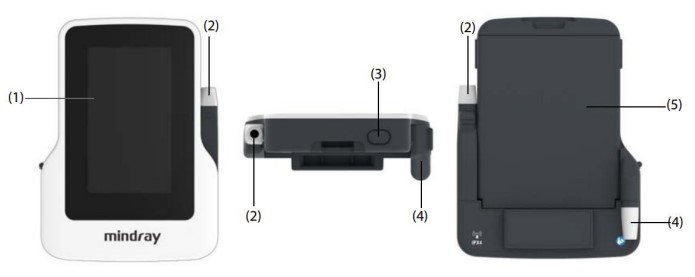
\includegraphics[width=.75\linewidth]{ePM15.jpg}
    \caption[迈瑞ePM 12M生理信号监护仪EP20模块外观]{迈瑞ePM 12M生理信号监护仪EP20模块外观}{\label{fig:ePM15}}
\end{figure}

本实验采集心电、脉搏波以及呼吸信号,采样率分别为500Hz,125Hz和60Hz。心电信号采用三导联电极进行采集,安装方式如\autoref{fig:ECGelctrode}所示。

其中RA安放在右锁骨中线下侧靠近右肩处,LA安放在左锁骨中线下侧靠近左肩处,LL安放在左下腹。选择平坦、干燥、肌肉较少的部位作为电极安放部位,并避开出血或破损的皮肤。安放电极前使用酒精棉片擦拭皮肤,
去除油性残渣及死皮细胞。电极安装好之后使用医用胶带进行固定。脉搏信号采用透射式血氧探头进行采集。测量部位为食指指尖,如果食指有损伤,则选择中指作为测量部位。测量时把手指放入指套内部,
指甲与传感器表面有指甲标记的部位正对,指尖触及但不超出指套顶端,确保发光管发出的所有光线全部通过被试的组织。佩戴方式如\autoref{fig:fingerelectrode}所示。

\begin{figure}[htbp]
    \hspace {0.1cm}
	\centering
	\begin{minipage}[l]{0.30\textwidth}
		% \hspace {-1cm}
        \centering
		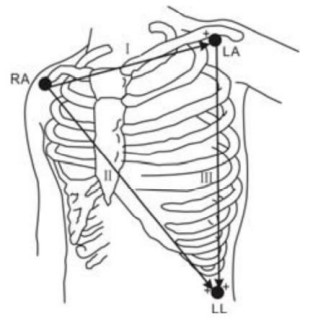
\includegraphics[width=0.9\textwidth]{ECGelctrode.jpg}
		\caption[心电电极安装示意图]{心电电极安装示意图}
		\label{fig:ECGelctrode}
	\end{minipage} 
    \hspace{.65in}
	\begin{minipage}[c]{0.4\textwidth}
		\hspace {-1cm}
        \centering
        \vspace{-1.5em}
        \setlength{\abovecaptionskip}{3em}
		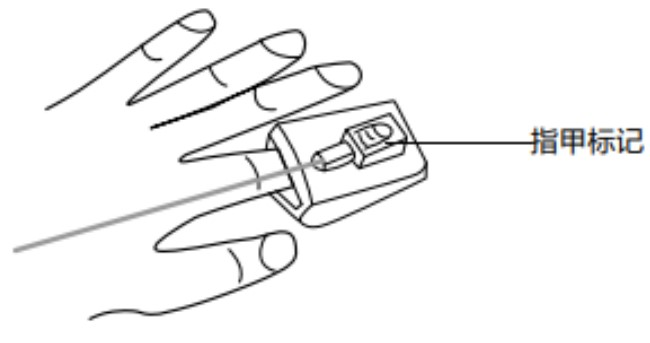
\includegraphics[width=\textwidth]{fingerelectrode.jpg}
        \caption[指夹佩戴示意图]{指夹佩戴示意图$\qquad$ $\qquad$ $\quad$ }
		\label{fig:fingerelectrode}
	\end{minipage}
\end{figure}

呼吸信号由监护仪使用阻抗法从心电信号中自动提取得到。
人的呼吸过程会造成胸腔的扩张和收缩,从而改变其电阻率,进而引起心电信号的周期性波动。采用傅里叶变换、小波变换或 FIR 滤波等方法获取这些规律性波形信息,即可从心电中提取呼吸信号。

实验时将EP20的腕带安放在被试的左手手腕,调整腕带长度并粘紧魔术贴,确保仪器位置固定但不会压迫被试的手腕。整体连接方式如\autoref{fig:allelectrode}所示,其中(1)为血氧传感器,(2)为腕带,(3)为EP20,(4)为ECGcable,(5)为心电电极。 
\begin{figure}[htbp]
    \centering
    \vspace{-0.2em}
    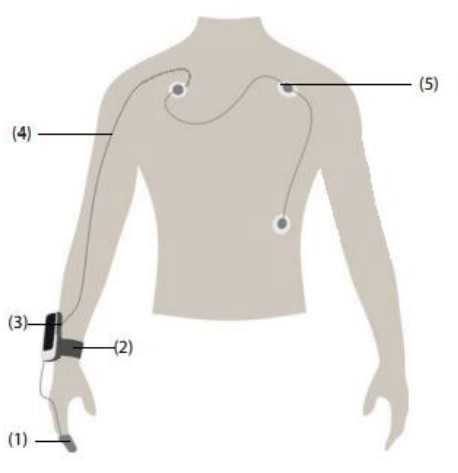
\includegraphics[width=.35\linewidth]{allelectrode.jpg}
    \setlength{\abovecaptionskip}{0.2em}
    \caption[信号采集仪器佩戴示意图]{信号采集仪器佩戴示意图}{\label{fig:allelectrode}}
\end{figure}

\subsubsection{数据处理与结果分析}
\begin{enumerate}[\hspace{2em}1.]
    \item 信号处理与特征提取、分析
\end{enumerate}

以20s为一段截取被试观看情绪视频时的生理数据,并根据视频片段所属情绪种类为数据打上标签,标明该段数据代表何种情绪。对有效数据进行预处理后,从时域、频域、非线性等多个维度提取多种特征参数并进行统计学分析(如相关性等),从中选出情绪识别的潜在有效特征,并对有效特征与生理变化的内在关联进行分析。

\begin{enumerate}[\hspace{2em}2.]
    \item 模型构建与验证
\end{enumerate}

使用机器学习方法(如支持向量机等算法)构建情绪识别模型,利用已有情绪标签的数据训练模型,尝试实现恐惧平静二分类,愉悦平静二分类和恐惧愉悦二分类,并从分类准确率、ROC曲线、AUC值等不同的角度对情绪识别模型的性能进行分析和评估。

\subsection{可行性分析}
% \subsubsection{心理学基础}
从心理学研究上看,继James-Lange情绪外周理论\cite{James1884}之后,任何情绪都伴随一定生理唤醒的观点在心理学界得到普遍认可,利用外周生理信号进行情绪识别研究具备充分的心理学理论基础。
论文选取的恐惧和愉悦情绪在主观体验上区别明显,依赖于个体的主观报告或量表检测能够反馈较好的区分结果,为数据处理和情绪诱发效果的评估提供有力支持。同时,在效价-唤醒度模型中,
恐惧和愉悦分属负价轴的消极情绪和正向轴的积极情绪,且效价绝对值大致相同,如在Hoffman等\cite{Hoffmann2012}的研究中,恐惧和愉悦的效价分别为-0.74和0.82。这样的特性对研究正负性情绪及其实验设计非常适用。

% \subsubsection{生理学基础}
从生理表现上看,恐惧和愉悦都能够引发人体较为明显的生理反应,与心电、脉搏和呼吸信号之间关系紧密。恐惧的特征是交感神经被激活,导致射血前期缩短,进而导致心率加速;同时心输出量增加,导致局部血流变化,血压升高,还伴随出汗、支气管扩张和由压力引起的过度换气等生理表现\cite{Curtis2002}。
愉悦则能够有效抵消前述部分生理变化,促使个体加速从高唤醒度情绪所引发的心血管反应增强、心率血压上升等生理反应中恢复基线水平。以上这些改变都很容易用生理信号的不同特征来表征,对情绪识别研究极为适用。
同时,在效价-唤醒度模型中,恐惧和愉悦分属负价轴的消极情绪和正向轴的积极情绪,且效价绝对值大致相同,如在Hoffman等的研究中,恐惧和愉悦的效价分别为-0.74和0.82。这样的特性对研究正负性情绪及其实验设计非常适用。

此外,论文采用的电影片段情绪诱发方式和自我评估量表等评价方式以及后续的统计学分析方法和机器学习方法,已经在大量研究中得到检验,具备良好的可行性。